\usetikzlibrary{calc}


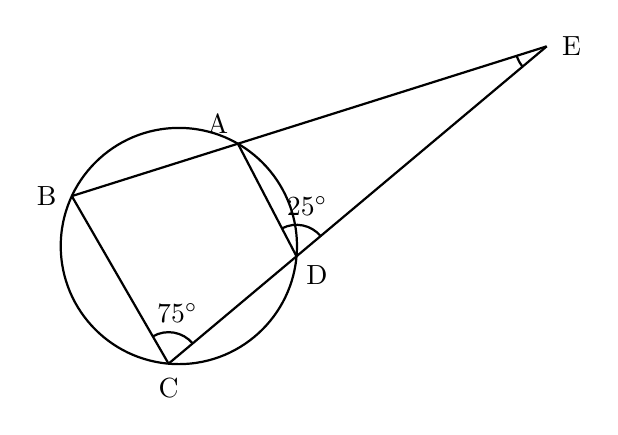
\begin{tikzpicture}[scale=1]

    % Define the center of the circle
    \coordinate (O) at (0,0);

    % Draw the circle
    \draw[thick] (O) circle (1.5);

    % Define points A, B, C, D on the circle based on calculated visual angles
    \coordinate (A) at (60:1.5);
    \coordinate (B) at (155:1.5);
    \coordinate (C) at (265:1.5);
    \coordinate (D) at (355:1.5);

    % Calculate intersection E of extended lines BA and CD
    \coordinate (E) at (intersection of B--A and C--D);

    % Draw the base of the cyclic quadrilateral and the segment AD
    \draw[thick] (B) -- (C);
    \draw[thick] (A) -- (D);

    % Draw the extended lines through A and D to E
    \draw[thick] (B) -- (E);
    \draw[thick] (C) -- (E);

    % Draw angle arc at C (Angle BCD)
    % Angle from C to D is approx 40 degrees, C to B is approx 120 degrees
    \draw[thick] (C) ++(40:0.4) arc (40:120:0.4);

    % Draw angle arc at D (Angle ADE, on the outside/other side of the chord)
    % Angle from D to E is approx 40 degrees, D to A is approx 117 degrees
    \draw[thick] (D) ++(40:0.4) arc (40:117:0.4);

    % Draw angle arc at E (Angle BEC)
    % Angle from E to B is approx 198 degrees, E to C is approx 220 degrees
    \draw[thick] (E) ++(198:0.4) arc (198:220:0.4);

    % Add labels for the points
    \node[above left] at (A) {A};
    \node[left, xshift=-2pt] at (B) {B};
    \node[below, yshift=-2pt] at (C) {C};
    \node[below right] at (D) {D};
    \node[right, xshift=2pt] at (E) {E};

    % Add angle values
    \node at ($(C) + (80:0.65)$) {$75^{\circ}$};
    \node at ($(D) + (78:0.65)$) {$25^{\circ}$};

\end{tikzpicture}